% Choose one to switch between slides and handout
%\documentclass[]{beamer}
\documentclass[handout]{beamer}

% Video Meta Data
\title{Bitcoin, Blockchain and Cryptoassets}
\subtitle{History of Digital Money}
\author{Prof. Dr. Fabian Schär}
\institute{University of Basel}

% Config File
% Packages
\usepackage[utf8]{inputenc}
\usepackage{hyperref}
\usepackage{gitinfo2}
\usepackage{tikz}
\usepackage{amsmath}
\usepackage{mathtools}
\usepackage{bibentry}
\usepackage{xcolor}
\usepackage{colortbl} % Add colour to LaTeX tables
\usepackage{caption}
\usepackage[export]{adjustbox}
\usepackage{pgfplots} \pgfplotsset{compat = 1.17}
\usepackage{makecell}
\usepackage{fancybox}
\usepackage{ragged2e}
\usepackage{fontawesome}
\usepackage{seqsplit}
\usepackage{tabularx}

% Color Options
\definecolor{highlight}{rgb}{0.65,0.84,0.82}
\definecolor{focus}{rgb}{0.72, 0, 0}
\definecolor{lightred}{rgb}{0.8,0.5,0.5}
\definecolor{midgray}{RGB}{190,195,200}

% Beamer Template Options
\beamertemplatenavigationsymbolsempty
\setbeamertemplate{footline}[frame number]
\setbeamercolor{structure}{fg=black}
\setbeamercolor{footline}{fg=black}
\setbeamercolor{title}{fg=black}
\setbeamercolor{frametitle}{fg=black}
\setbeamercolor{item}{fg=black}
\setbeamercolor{}{fg=black}
\setbeamercolor{bibliography item}{fg=black}
\setbeamercolor*{bibliography entry title}{fg=black}
\setbeamercolor{alerted text}{fg=focus}
\setbeamertemplate{items}[square]
\setbeamertemplate{enumerate items}[default]
\captionsetup[figure]{labelfont={color=black},font={color=black}}
\captionsetup[table]{labelfont={color=black},font={color=black}}

\setbeamertemplate{bibliography item}{\insertbiblabel}

% Link Icon Command
\newcommand{\link}{%
    \tikz[x=1.2ex, y=1.2ex, baseline=-0.05ex]{%
        \begin{scope}[x=1ex, y=1ex]
            \clip (-0.1,-0.1)
                --++ (-0, 1.2)
                --++ (0.6, 0)
                --++ (0, -0.6)
                --++ (0.6, 0)
                --++ (0, -1);
            \path[draw,
                line width = 0.5,
                rounded corners=0.5]
                (0,0) rectangle (1,1);
        \end{scope}
        \path[draw, line width = 0.5] (0.5, 0.5)
            -- (1, 1);
        \path[draw, line width = 0.5] (0.6, 1)
            -- (1, 1) -- (1, 0.6);
        }
    }

% Read Git Data from Github Actions Workflow
% Defaults to gitinfo2 for local builds
\IfFileExists{gitInfo.txt}
	{\input{gitInfo.txt}}
	{
		\newcommand{\gitRelease}{(Local Release)}
		\newcommand{\gitSHA}{\gitHash}
		\newcommand{\gitDate}{\gitAuthorIsoDate}
	}

% Custom Titlepage
\defbeamertemplate*{title page}{customized}[1][]
{
  \vspace{-0cm}\hfill\includegraphics[width=2.5cm]{../config/logo_cif}
  \includegraphics[width=1.9cm]{../config/seal_wwz}
  \\ \vspace{2em}
  \usebeamerfont{title}\textbf{\inserttitle}\par
  \usebeamerfont{title}\usebeamercolor[fg]{title}\insertsubtitle\par  \vspace{1.5em}
  \small\usebeamerfont{author}\insertauthor\par
  \usebeamerfont{author}\insertinstitute\par \vspace{2em}
  \usebeamercolor[fg]{titlegraphic}\inserttitlegraphic
    \tiny \noindent \texttt{Release Ver.: \gitRelease}\\ 
    \texttt{Version Hash: \gitSHA}\\
    \texttt{Version Date: \gitDate}\\ \vspace{1em}
    
    
    \iffalse
  \link \href{https://github.com/cifunibas/Bitcoin-Blockchain-Cryptoassets/blob/main/slides/intro.pdf}
  {Get most recent version}\\
  \link \href{https://github.com/cifunibas/Bitcoin-Blockchain-Cryptoassets/blob/main/slides/intro.pdf}
  {Watch video lecture}\\ 
  
  \fi
  
  \vspace{1em}
  License: \texttt{Creative Commons Attribution-NonCommercial-ShareAlike 4.0 International}\\\vspace{2em}
  \includegraphics[width = 1.2cm]{../config/license}
}


% tikzlibraries
\usetikzlibrary{decorations.pathreplacing}
\usetikzlibrary{decorations.markings}
\usetikzlibrary{positioning}
\usetikzlibrary{calc}
\captionsetup{font=footnotesize}


%%%%%%%%%%%%%%%%%%%%%%%%%%%%%%%%%%%%%%%%%%%%%%
%%%%%%%%%%%%%%%%%%%%%%%%%%%%%%%%%%%%%%%%%%%%%%
\begin{document}

\thispagestyle{empty}
\begin{frame}[noframenumbering]
	\titlepage
\end{frame}



%%%
\begin{frame}{Before Bitcoin}
\begin{columns}
	\column{0.4\textwidth}
		\begin{figure}
			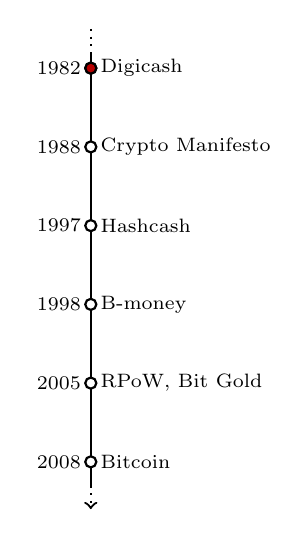
\begin{tikzpicture}[scale=1]
						%draw vertical line
		%\draw [thick] (0,4) -- (0,2.3);
		%\draw [thick,dotted] (0,2.3) -- (0,1.7);
		%\draw [thick] (0,1.7) -- (0,0.3);
		%\draw [thick,dotted] (0,0.3) -- (0,-0.3);
		%\draw [thick, ->] (0,-0.3) -- (0,-2);
		\draw [thick,dotted] (0,4) -- (0,3.7);
		\draw [thick] (0,3.7) -- (0,-1.8);
		\draw [thick,dotted, ->] (0,-1.8) -- (0,-2.1);
		
		%draw bullet points
		\foreach \x in {3.5,2.5,1.5,0.5,-0.5,-1.5}
		\filldraw[draw=black, fill = white, thick] (0, \x cm) circle (2pt);
		
		
		%years & names
		\draw(0,3.5) node[left] {{\scriptsize 1982}} node[right] {{\scriptsize Digicash}};
		\draw(0,2.5) node[left] {{\scriptsize 1988}} node[right] {{\scriptsize Crypto Manifesto}};
		\draw(0,1.5) node[left] {{\scriptsize 1997}} node[right] {{\scriptsize Hashcash}};
		\draw(0,0.5) node[left] {{\scriptsize 1998}} node[right] {{\scriptsize B-money}};
		\draw(0,-0.5) node[left] {{\scriptsize 2005}} node[right] {{\scriptsize RPoW, Bit Gold}};
		\draw(0,-1.5) node[left] {{\scriptsize 2008}} node[right] {{\scriptsize Bitcoin}};

				\filldraw[draw=black, fill = focus, thick] (0, 3.5 cm) circle (2pt);
			\end{tikzpicture}
		\end{figure}
	\column{0.7\textwidth}
		\textbf{Digicash - David Chaum}
		\vspace{0.5em}
		\begin{small}
		\begin{itemize}
			\item Concern: Electronic means of payment significantly limit privacy and traceable payment flows may generate sensitive data.
			\item Goal: Virtual monetary unit that imitates the anonymity of cash.
			\item Monopolized money creation and centralized settlement.
			\item Central bank blindly signs monetary units.
		\end{itemize}
		\end{small}	
\end{columns}
\end{frame}
%%%


%%%
\begin{frame}{Before Bitcoin}
\begin{columns}
	\column{0.4\textwidth}
		\begin{figure}
			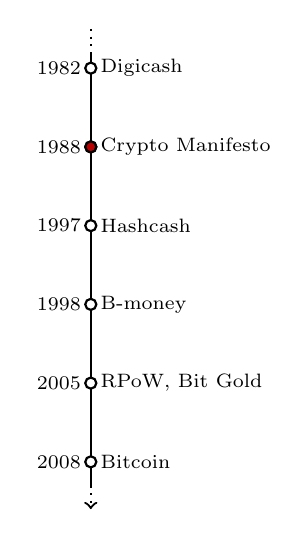
\begin{tikzpicture}[scale=1]
						%draw vertical line
		%\draw [thick] (0,4) -- (0,2.3);
		%\draw [thick,dotted] (0,2.3) -- (0,1.7);
		%\draw [thick] (0,1.7) -- (0,0.3);
		%\draw [thick,dotted] (0,0.3) -- (0,-0.3);
		%\draw [thick, ->] (0,-0.3) -- (0,-2);
		\draw [thick,dotted] (0,4) -- (0,3.7);
		\draw [thick] (0,3.7) -- (0,-1.8);
		\draw [thick,dotted, ->] (0,-1.8) -- (0,-2.1);
		
		%draw bullet points
		\foreach \x in {3.5,2.5,1.5,0.5,-0.5,-1.5}
		\filldraw[draw=black, fill = white, thick] (0, \x cm) circle (2pt);
		
		
		%years & names
		\draw(0,3.5) node[left] {{\scriptsize 1982}} node[right] {{\scriptsize Digicash}};
		\draw(0,2.5) node[left] {{\scriptsize 1988}} node[right] {{\scriptsize Crypto Manifesto}};
		\draw(0,1.5) node[left] {{\scriptsize 1997}} node[right] {{\scriptsize Hashcash}};
		\draw(0,0.5) node[left] {{\scriptsize 1998}} node[right] {{\scriptsize B-money}};
		\draw(0,-0.5) node[left] {{\scriptsize 2005}} node[right] {{\scriptsize RPoW, Bit Gold}};
		\draw(0,-1.5) node[left] {{\scriptsize 2008}} node[right] {{\scriptsize Bitcoin}};

				\filldraw[draw=black, fill = focus, thick] (0, 2.5 cm) circle (2pt);	
			\end{tikzpicture}
		\end{figure}
	\column{0.7\textwidth}
		\textbf{Crypto Anarchist Manifesto - Tim May} \\
		\vspace{0.5em}
		\link \href{https://groups.csail.mit.edu/mac/classes/6.805/articles/crypto/cypherpunks/may-crypto-manifesto.html}{Link} \\
		\vspace{0.5em}
		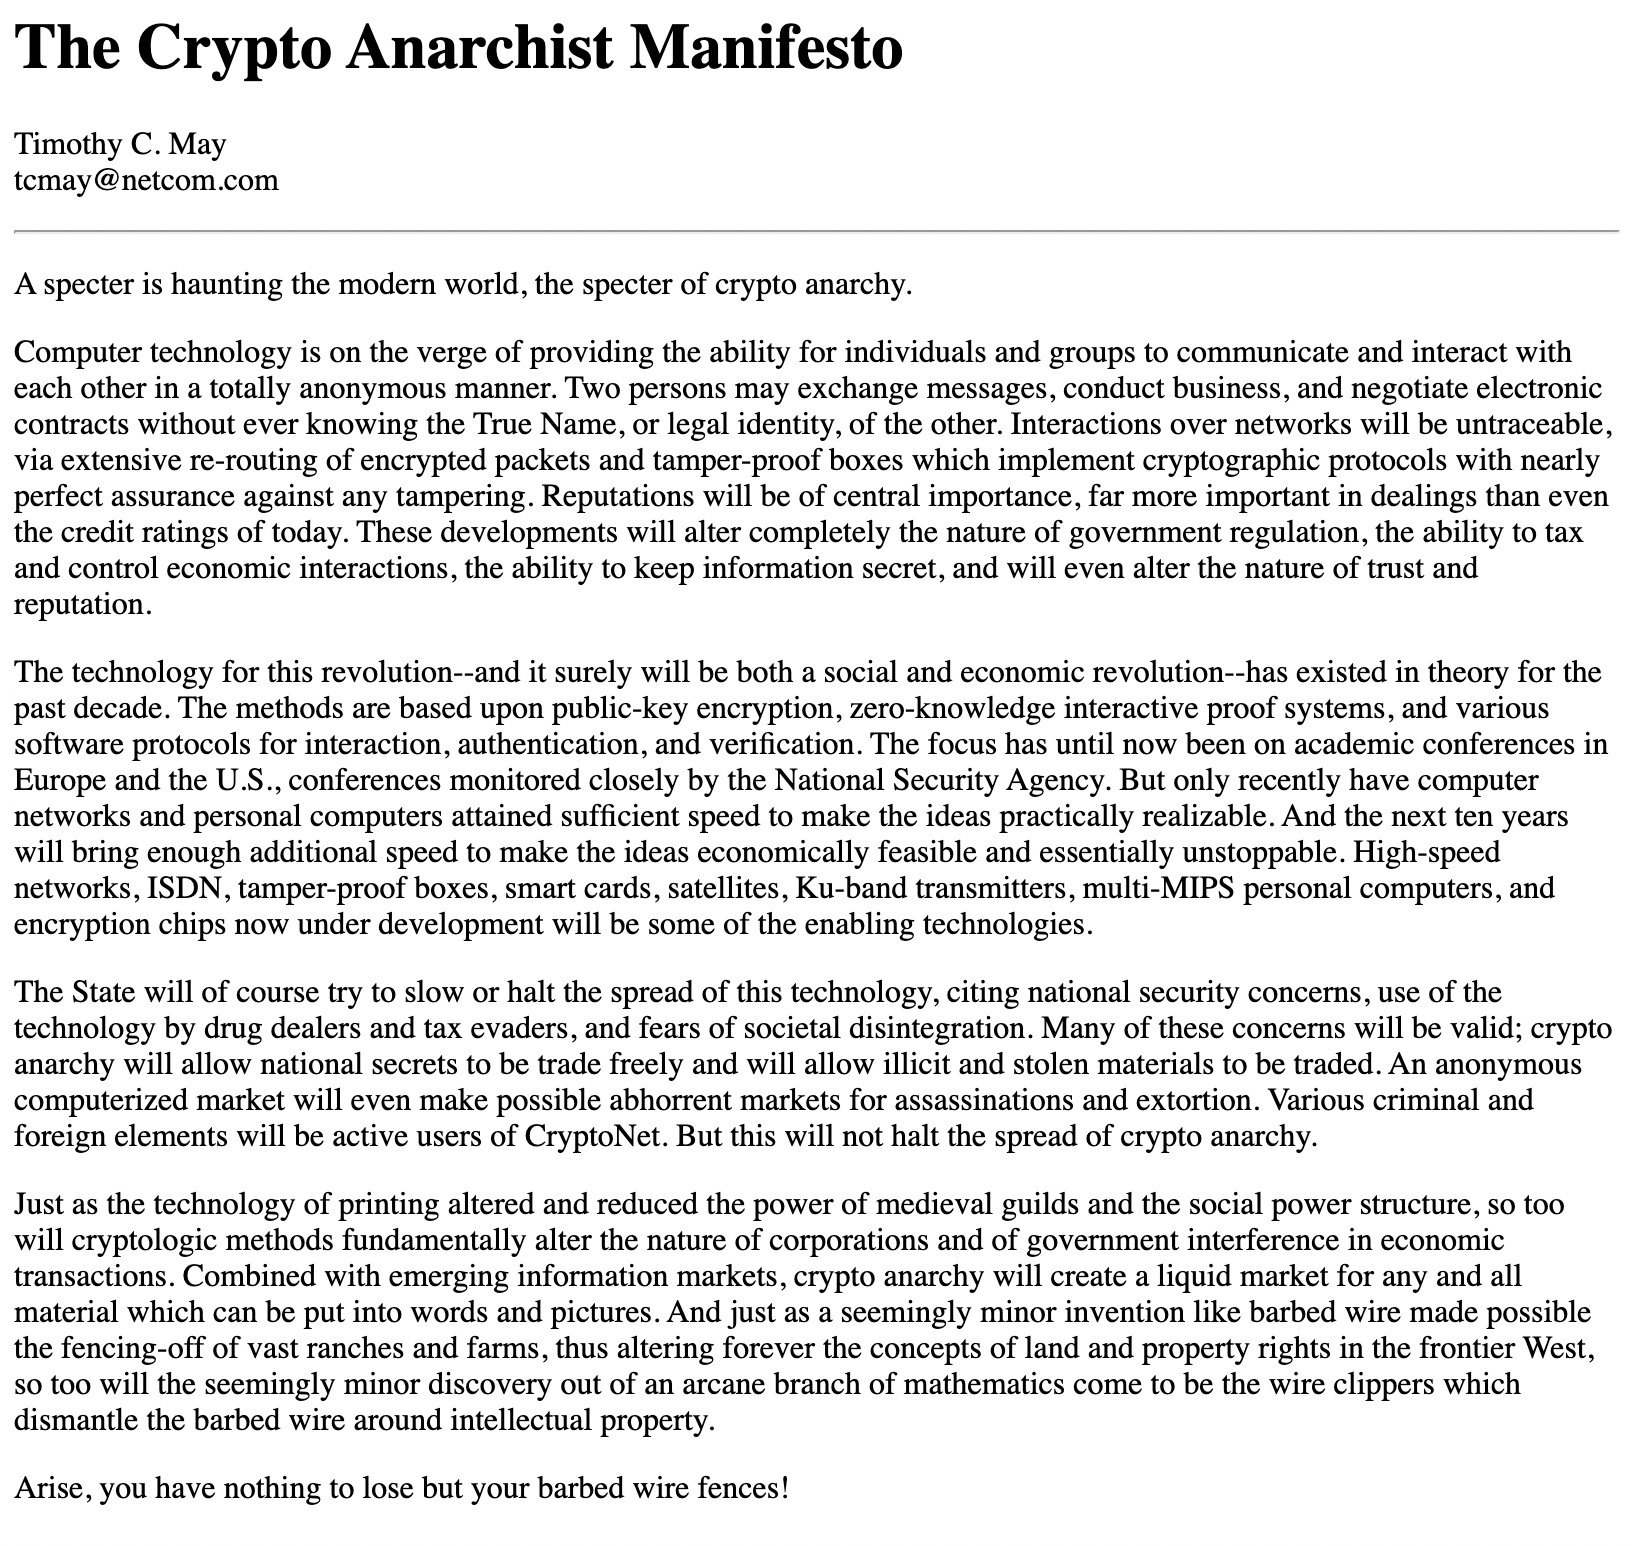
\includegraphics[scale=0.23]{../assets/images/crypto_manifesto}
\end{columns}
\end{frame}
%%%


%%%
\begin{frame}{Before Bitcoin}
\begin{columns}
\column{0.4\textwidth}
\begin{figure}
	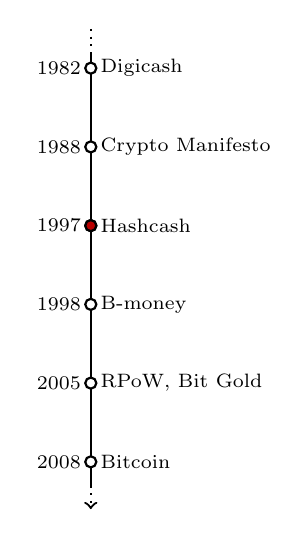
\begin{tikzpicture}[scale=1]
				%draw vertical line
		%\draw [thick] (0,4) -- (0,2.3);
		%\draw [thick,dotted] (0,2.3) -- (0,1.7);
		%\draw [thick] (0,1.7) -- (0,0.3);
		%\draw [thick,dotted] (0,0.3) -- (0,-0.3);
		%\draw [thick, ->] (0,-0.3) -- (0,-2);
		\draw [thick,dotted] (0,4) -- (0,3.7);
		\draw [thick] (0,3.7) -- (0,-1.8);
		\draw [thick,dotted, ->] (0,-1.8) -- (0,-2.1);
		
		%draw bullet points
		\foreach \x in {3.5,2.5,1.5,0.5,-0.5,-1.5}
		\filldraw[draw=black, fill = white, thick] (0, \x cm) circle (2pt);
		
		
		%years & names
		\draw(0,3.5) node[left] {{\scriptsize 1982}} node[right] {{\scriptsize Digicash}};
		\draw(0,2.5) node[left] {{\scriptsize 1988}} node[right] {{\scriptsize Crypto Manifesto}};
		\draw(0,1.5) node[left] {{\scriptsize 1997}} node[right] {{\scriptsize Hashcash}};
		\draw(0,0.5) node[left] {{\scriptsize 1998}} node[right] {{\scriptsize B-money}};
		\draw(0,-0.5) node[left] {{\scriptsize 2005}} node[right] {{\scriptsize RPoW, Bit Gold}};
		\draw(0,-1.5) node[left] {{\scriptsize 2008}} node[right] {{\scriptsize Bitcoin}};

		\filldraw[draw=black, fill = focus, thick] (0, 1.5 cm) circle (2pt);	
	\end{tikzpicture}
\end{figure}
\column{0.7\textwidth}
	\textbf{Hashcash - Adam Back}
	\vspace{0.5em}
	\begin{small}
	\begin{itemize}
		\item Originally proposed as a mechanism for anti-DoS and spam email.
		\item Introduced concept of artificial costs.
		\item "The idea of using partial hashes is that they can be made arbitrarily expensive to compute (by choosing the desired number of bits of collision), and yet can be verified instantly." \cite{back2002}
	\end{itemize}
	\end{small}
\end{columns}
\end{frame}
%%%	


%%%
\begin{frame}{Before Bitcoin}
\begin{columns}
\column{0.4\textwidth}
\begin{figure}
	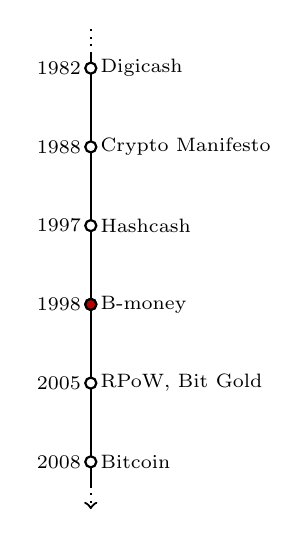
\begin{tikzpicture}[scale=1]
				%draw vertical line
		%\draw [thick] (0,4) -- (0,2.3);
		%\draw [thick,dotted] (0,2.3) -- (0,1.7);
		%\draw [thick] (0,1.7) -- (0,0.3);
		%\draw [thick,dotted] (0,0.3) -- (0,-0.3);
		%\draw [thick, ->] (0,-0.3) -- (0,-2);
		\draw [thick,dotted] (0,4) -- (0,3.7);
		\draw [thick] (0,3.7) -- (0,-1.8);
		\draw [thick,dotted, ->] (0,-1.8) -- (0,-2.1);
		
		%draw bullet points
		\foreach \x in {3.5,2.5,1.5,0.5,-0.5,-1.5}
		\filldraw[draw=black, fill = white, thick] (0, \x cm) circle (2pt);
		
		
		%years & names
		\draw(0,3.5) node[left] {{\scriptsize 1982}} node[right] {{\scriptsize Digicash}};
		\draw(0,2.5) node[left] {{\scriptsize 1988}} node[right] {{\scriptsize Crypto Manifesto}};
		\draw(0,1.5) node[left] {{\scriptsize 1997}} node[right] {{\scriptsize Hashcash}};
		\draw(0,0.5) node[left] {{\scriptsize 1998}} node[right] {{\scriptsize B-money}};
		\draw(0,-0.5) node[left] {{\scriptsize 2005}} node[right] {{\scriptsize RPoW, Bit Gold}};
		\draw(0,-1.5) node[left] {{\scriptsize 2008}} node[right] {{\scriptsize Bitcoin}};

		\filldraw[draw=black, fill = focus, thick] (0, 0.5 cm) circle (2pt);	
	\end{tikzpicture}
\end{figure}
\column{0.7\textwidth}
	\textbf{B-money - Wei Dai} \\
	\vspace{0.5em}
	\begin{small}
	\begin{itemize}
		\item Thought experiment
		\item Assumption: Existence of an untraceable network.
		\item Senders and receivers are identified only by digital pseudonyms. (i.e. public keys) 
		\item Transaction legitimacy guaranteed by signature with associated private key.
		\item Participants keep separate registers with the current balances of all pseudonyms.
		\item Competitive money creation by solving numerical puzzles that are hard to compute but easy to verify.
	\end{itemize}
	\end{small}
\end{columns}
\end{frame}
%%%	


%%%
\begin{frame}{Before Bitcoin}
\begin{columns}
\column{0.4\textwidth}
\begin{figure}
	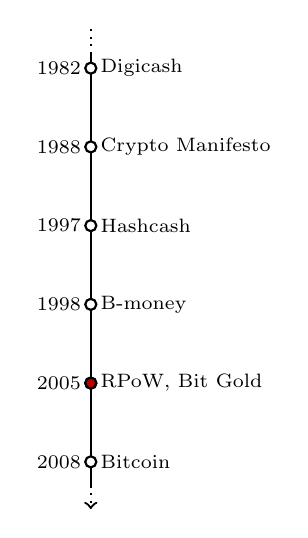
\begin{tikzpicture}[scale=1]
				%draw vertical line
		%\draw [thick] (0,4) -- (0,2.3);
		%\draw [thick,dotted] (0,2.3) -- (0,1.7);
		%\draw [thick] (0,1.7) -- (0,0.3);
		%\draw [thick,dotted] (0,0.3) -- (0,-0.3);
		%\draw [thick, ->] (0,-0.3) -- (0,-2);
		\draw [thick,dotted] (0,4) -- (0,3.7);
		\draw [thick] (0,3.7) -- (0,-1.8);
		\draw [thick,dotted, ->] (0,-1.8) -- (0,-2.1);
		
		%draw bullet points
		\foreach \x in {3.5,2.5,1.5,0.5,-0.5,-1.5}
		\filldraw[draw=black, fill = white, thick] (0, \x cm) circle (2pt);
		
		
		%years & names
		\draw(0,3.5) node[left] {{\scriptsize 1982}} node[right] {{\scriptsize Digicash}};
		\draw(0,2.5) node[left] {{\scriptsize 1988}} node[right] {{\scriptsize Crypto Manifesto}};
		\draw(0,1.5) node[left] {{\scriptsize 1997}} node[right] {{\scriptsize Hashcash}};
		\draw(0,0.5) node[left] {{\scriptsize 1998}} node[right] {{\scriptsize B-money}};
		\draw(0,-0.5) node[left] {{\scriptsize 2005}} node[right] {{\scriptsize RPoW, Bit Gold}};
		\draw(0,-1.5) node[left] {{\scriptsize 2008}} node[right] {{\scriptsize Bitcoin}};

		\filldraw[draw=black, fill = focus, thick] (0, -0.5 cm) circle (2pt);	
	\end{tikzpicture}
\end{figure}
\column{0.7\textwidth}
	\textbf{Reusable Proofs of Work - Hal Finney} \cite{finney2005}
	\vspace{0.5em}
	\begin{small}
	\begin{itemize}
		\item Combines ideas of Wei Dai and Adam Back.
		\item A RPoW client can create a RPoW token by providing a proof-of-work string and signing with his private key.
		\item Server can map that token to the signing key.
		\item Client can give the token to another key by signing a transfer order to a public key.
		\item Server registers the token as belonging to the corresponding private key.
	\end{itemize}
	\end{small}
\end{columns}
\end{frame}
%%%	


%%%
\begin{frame}{Before Bitcoin}
\begin{columns}
\column{0.4\textwidth}
\begin{figure}
	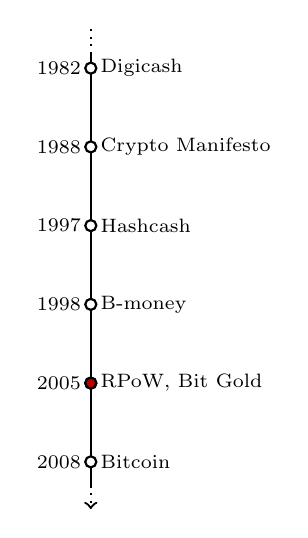
\begin{tikzpicture}[scale=1]
				%draw vertical line
		%\draw [thick] (0,4) -- (0,2.3);
		%\draw [thick,dotted] (0,2.3) -- (0,1.7);
		%\draw [thick] (0,1.7) -- (0,0.3);
		%\draw [thick,dotted] (0,0.3) -- (0,-0.3);
		%\draw [thick, ->] (0,-0.3) -- (0,-2);
		\draw [thick,dotted] (0,4) -- (0,3.7);
		\draw [thick] (0,3.7) -- (0,-1.8);
		\draw [thick,dotted, ->] (0,-1.8) -- (0,-2.1);
		
		%draw bullet points
		\foreach \x in {3.5,2.5,1.5,0.5,-0.5,-1.5}
		\filldraw[draw=black, fill = white, thick] (0, \x cm) circle (2pt);
		
		
		%years & names
		\draw(0,3.5) node[left] {{\scriptsize 1982}} node[right] {{\scriptsize Digicash}};
		\draw(0,2.5) node[left] {{\scriptsize 1988}} node[right] {{\scriptsize Crypto Manifesto}};
		\draw(0,1.5) node[left] {{\scriptsize 1997}} node[right] {{\scriptsize Hashcash}};
		\draw(0,0.5) node[left] {{\scriptsize 1998}} node[right] {{\scriptsize B-money}};
		\draw(0,-0.5) node[left] {{\scriptsize 2005}} node[right] {{\scriptsize RPoW, Bit Gold}};
		\draw(0,-1.5) node[left] {{\scriptsize 2008}} node[right] {{\scriptsize Bitcoin}};

		\filldraw[draw=black, fill = focus, thick] (0, -0.5 cm) circle (2pt);
	\end{tikzpicture}
\end{figure}
\column{0.7\textwidth}
	\textbf{Bit Gold - Nick Szabo}
	\vspace{0.5em}
	\begin{small}
	\begin{itemize}
		\item Describes the combination of the proof-of-work algorithm for competitive money creation.
		\item Computing power is used to collateralise a public ledger, which grows into a chain of blocks through a reflexive reference.
		\item "Thus, it would be very nice if there were a protocol whereby unforgeably costly bits could be created online with minimal dependence on trusted third parties, and then securely stored, transferred, and assayed with similar minimal trust. Bit gold." \cite{szabo2005}
	\end{itemize}
	\end{small}
\end{columns}
\end{frame}
%%%	

%%%
\begin{frame}%[allowframebreaks]

\frametitle{References and Recommended Reading}
	\bibliographystyle{amsplain}
	\bibliography{../assets/bib/refs}
\end{frame}
%%%

\end{document}

